\documentclass[11pt,a4paper]{article}
\usepackage[utf8]{inputenc}
\usepackage[spanish]{babel}
\usepackage{amsmath}
\usepackage{amsfonts}
\usepackage{amssymb}
\usepackage{graphicx}
\usepackage[margin=2.5cm]{geometry}
\usepackage{float}
\usepackage{cite}
\usepackage{url}

% Información del documento
\title{Simulación de Percolación en Redes 2D\\
       Análisis del Algoritmo de Hoshen-Kopelman}
\author{Tu Nombre\\
        Universidad Nacional de Colombia}
\date{\today}

\begin{document}

\maketitle

\begin{abstract}
Este trabajo presenta una implementación computacional del proceso de percolación en redes bidimensionales utilizando el algoritmo de Hoshen-Kopelman. Se analizaron sistemas de diferentes tamaños ($L = 32, 64, 128, 256, 512$) para estudiar el comportamiento crítico cerca del umbral de percolación $p_c \approx 0.5927$. Los resultados muestran la formación de clusters percolantes y la dependencia del tamaño del sistema en las propiedades críticas.
\end{abstract}

\section{Introducción}

La teoría de percolación es un área fundamental de la física estadística que estudia la conectividad en sistemas aleatorios \cite{stauffer1994introduction}. El problema clásico de percolación de sitios en una red cuadrada consiste en ocupar cada sitio independientemente con probabilidad $p$, y determinar si existe un camino conectado que atraviese todo el sistema \cite{grimmett1999percolation}.

El umbral de percolación crítico para una red cuadrada bidimensional es $p_c = 0.592746...$, valor que ha sido determinado con alta precisión tanto analítica como numéricamente \cite{kesten1980critical}. Cerca de este valor crítico, el sistema exhibe comportamiento de escala caracterizado por exponentes críticos universales.

\section{Metodología}

\subsection{Algoritmo de Hoshen-Kopelman}

Para identificar eficientemente los clusters conectados, implementamos el algoritmo de Hoshen-\linebreak Kopelman \cite{hoshen1976percolation}, que utiliza una estructura de datos Union-Find para mantener la conectividad de los sitios ocupados. Este algoritmo tiene complejidad temporal $O(N \alpha(N))$, donde $\alpha$ es la función inversa de Ackermann.

El algoritmo procede de la siguiente manera:
\begin{enumerate}
    \item Recorrer la red sitio por sitio
    \item Para cada sitio ocupado, verificar vecinos ya procesados
    \item Asignar etiqueta de cluster según conectividad
    \item Usar Union-Find para manejar fusiones de clusters
\end{enumerate}

\subsection{Parámetros de Simulación}

Se realizaron simulaciones para tamaños de red $L \in \{32, 64, 128, 256, 512\}$ y probabilidades en el rango $p \in [0.4, 0.8]$ con incrementos de $\Delta p = 0.01$. Para cada configuración se promediaron $N_{\text{samples}} = 1000$ realizaciones independientes.

\section{Resultados}

\subsection{Probabilidad de Percolación}

La Figura \ref{fig:percolation_prob} muestra la probabilidad de percolación $P(p,L)$ como función de $p$ para diferentes tamaños de sistema. Se observa una transición abrupta cerca de $p_c$, que se vuelve más pronunciada para sistemas más grandes.

\begin{figure}[H]
    \centering
    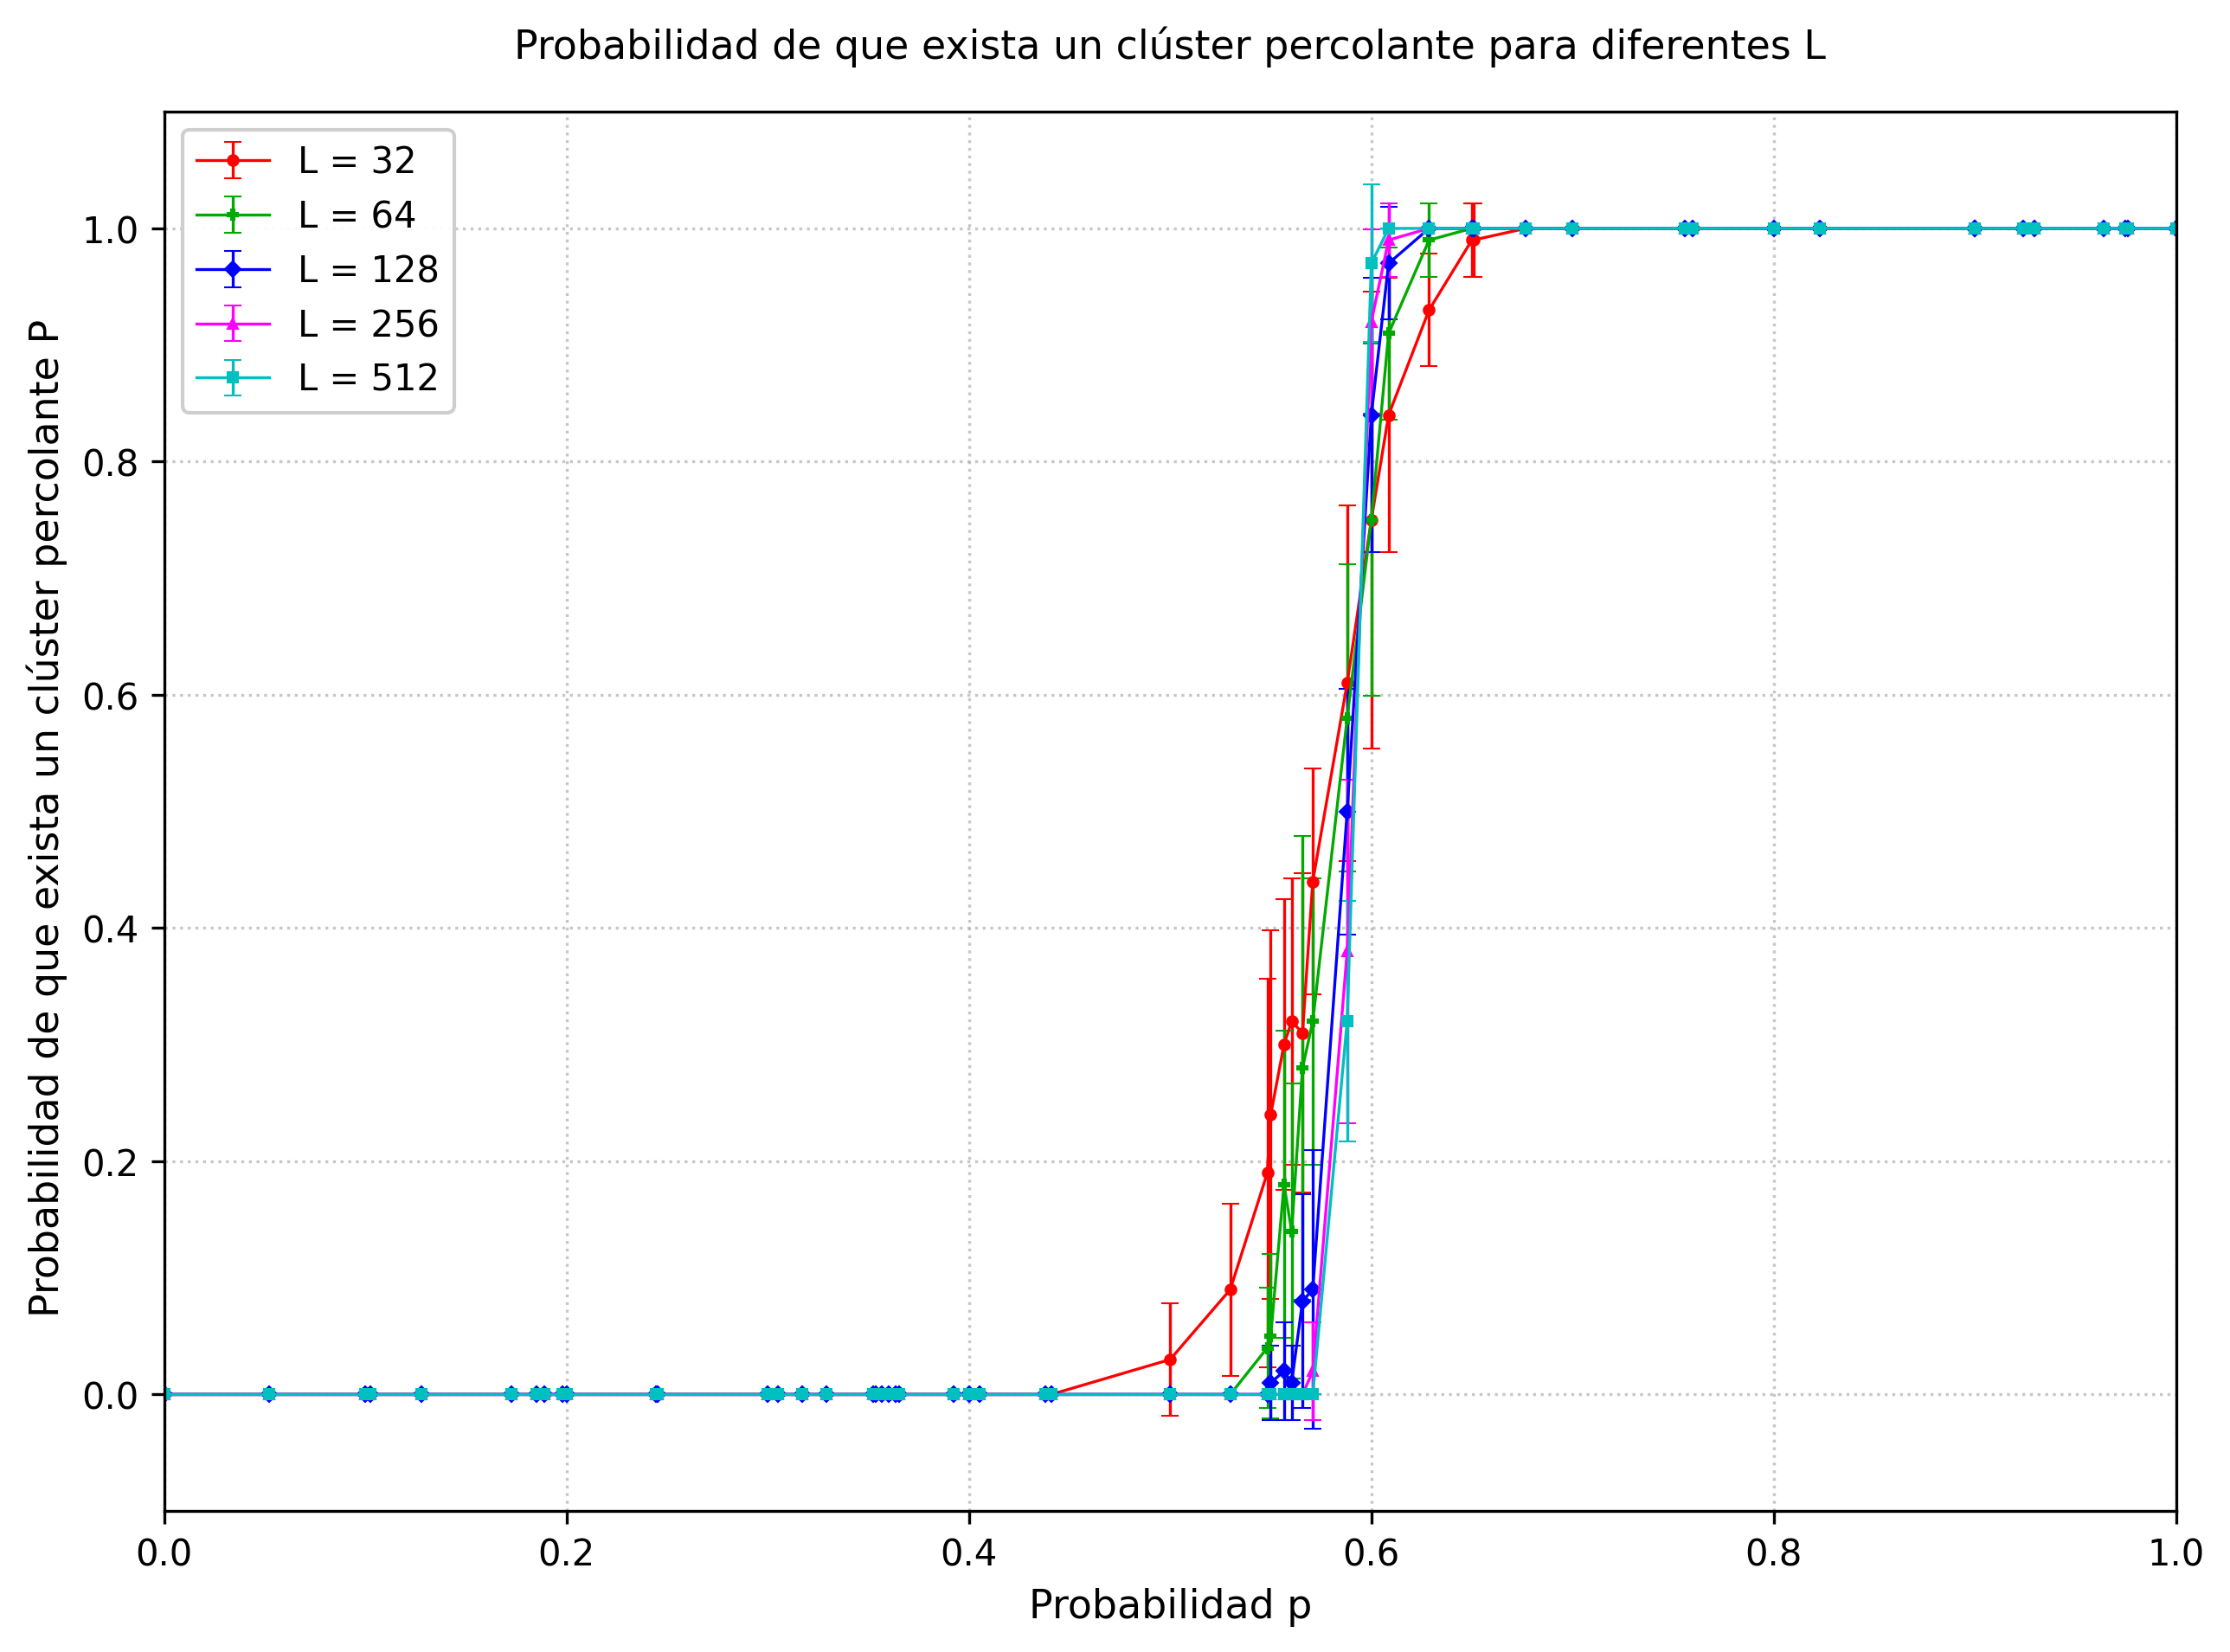
\includegraphics[width=0.8\textwidth]{../figures/P_all_L.png}
    \caption{Probabilidad de percolación $P(p,L)$ en función de $p$ para diferentes tamaños de red $L$. La transición se vuelve más abrupta al aumentar $L$.}
    \label{fig:percolation_prob}
\end{figure}

\subsection{Tamaño del Cluster Percolante}

El tamaño relativo del cluster percolante $S(p,L)$ se muestra en la Figura \ref{fig:cluster_size}. Para $p > p_c$, este tamaño escala aproximadamente como $(p - p_c)^{\beta}$ donde $\beta \approx 5/36$ es el exponente crítico teórico \cite{stauffer1994introduction}.

\begin{figure}[H]
    \centering
    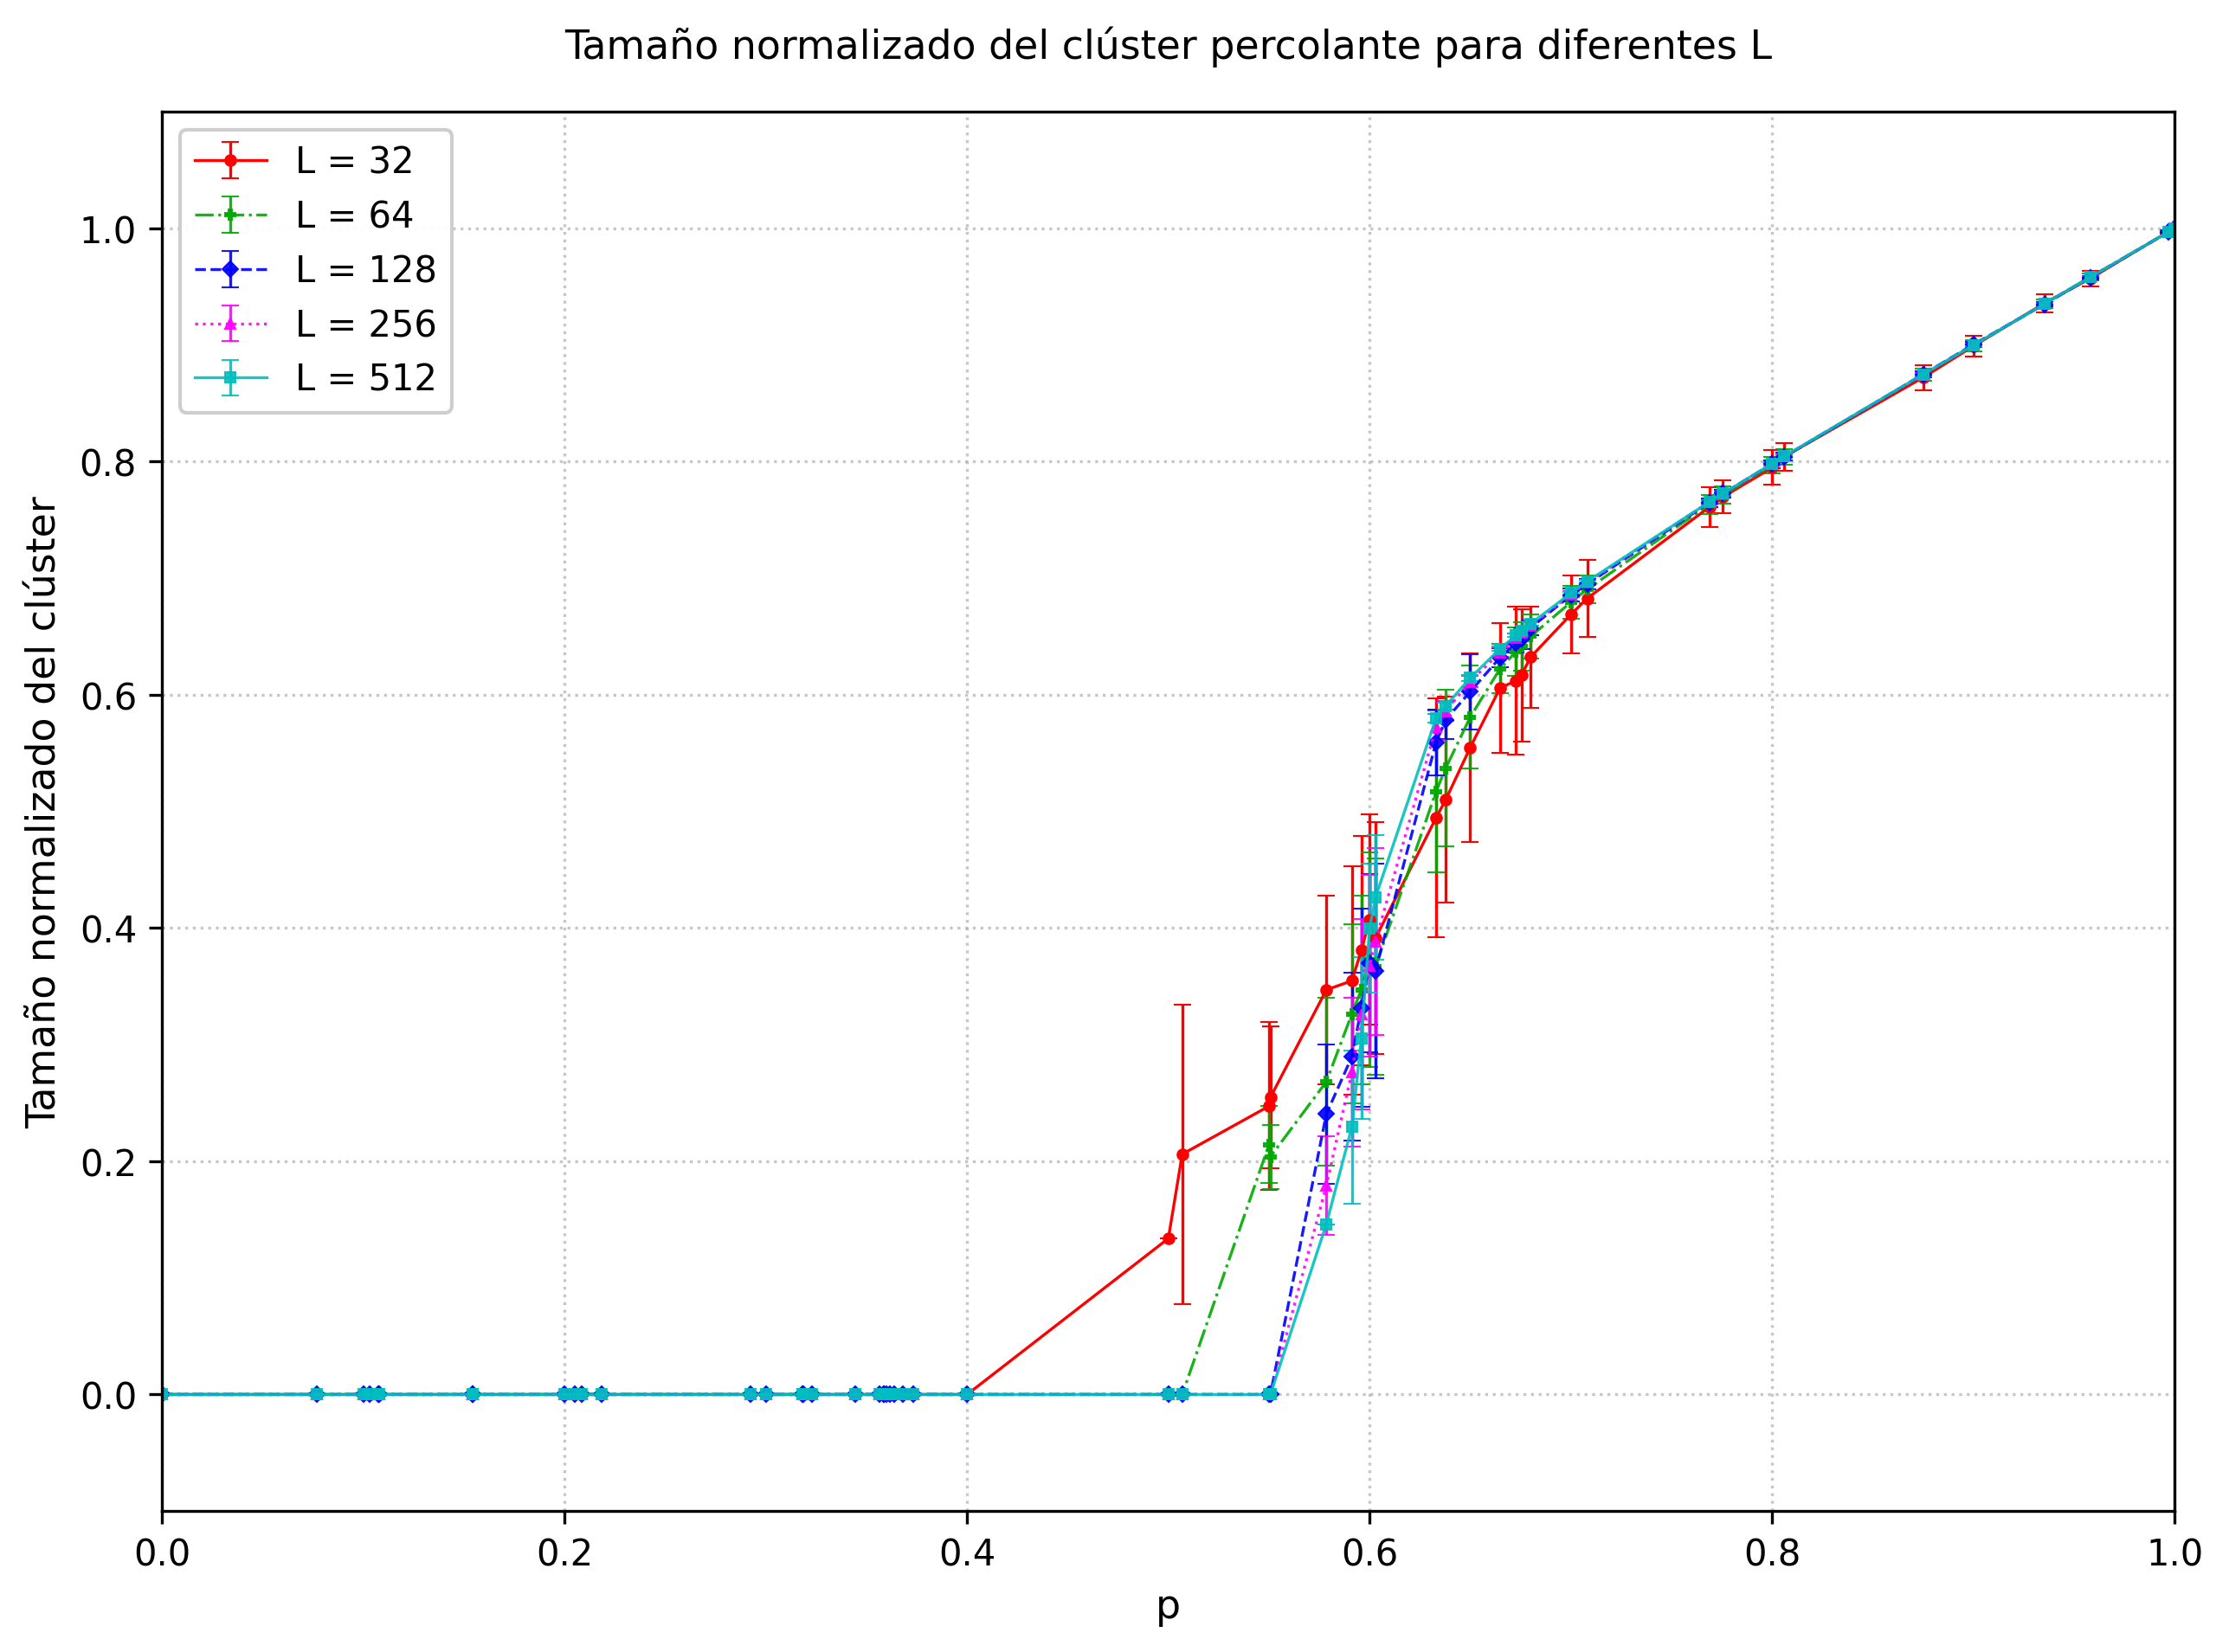
\includegraphics[width=0.8\textwidth]{../figures/Cluster_all_L.png}
    \caption{Tamaño relativo del cluster percolante $S(p,L)$ como función de $p$. Se observa el comportamiento de ley de potencias cerca del punto crítico.}
    \label{fig:cluster_size}
\end{figure}

\subsection{Visualización de Clusters}

Las Figuras \ref{fig:visualization} y \ref{fig:cluster_vis} muestran configuraciones típicas del sistema para diferentes valores de $p$, ilustrando la formación y evolución de clusters conectados.

\begin{figure}[H]
    \centering
    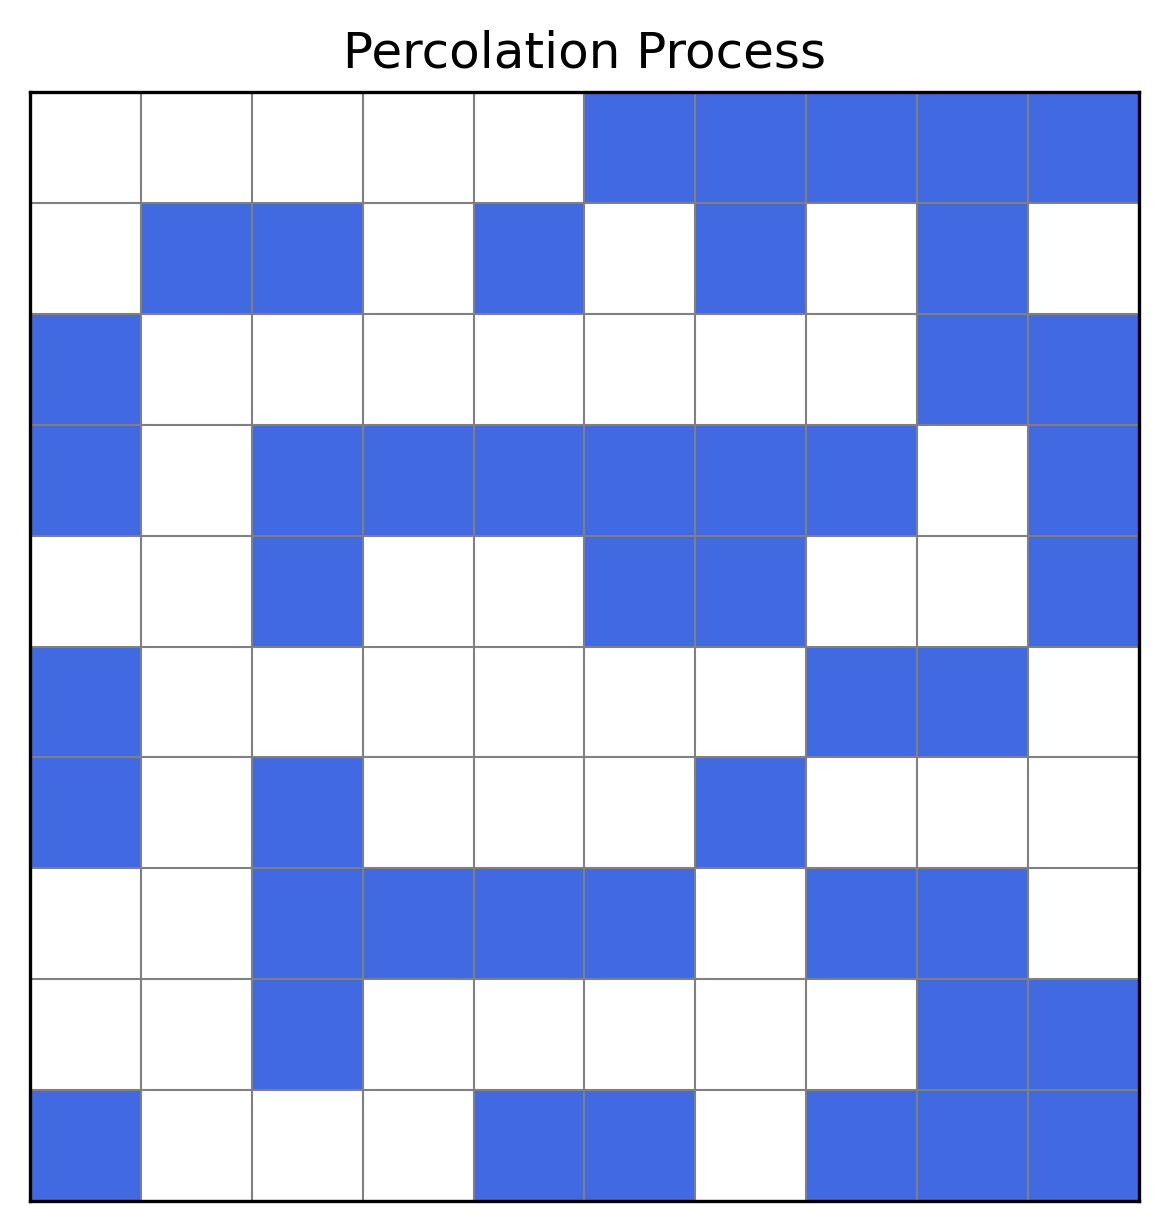
\includegraphics[width=0.7\textwidth]{../figures/percolation.png}
    \caption{Visualización de una configuración típica de percolación mostrando sitios ocupados (negro) y vacíos (blanco) para $p = 0.6$.}
    \label{fig:visualization}
\end{figure}

\begin{figure}[H]
    \centering
    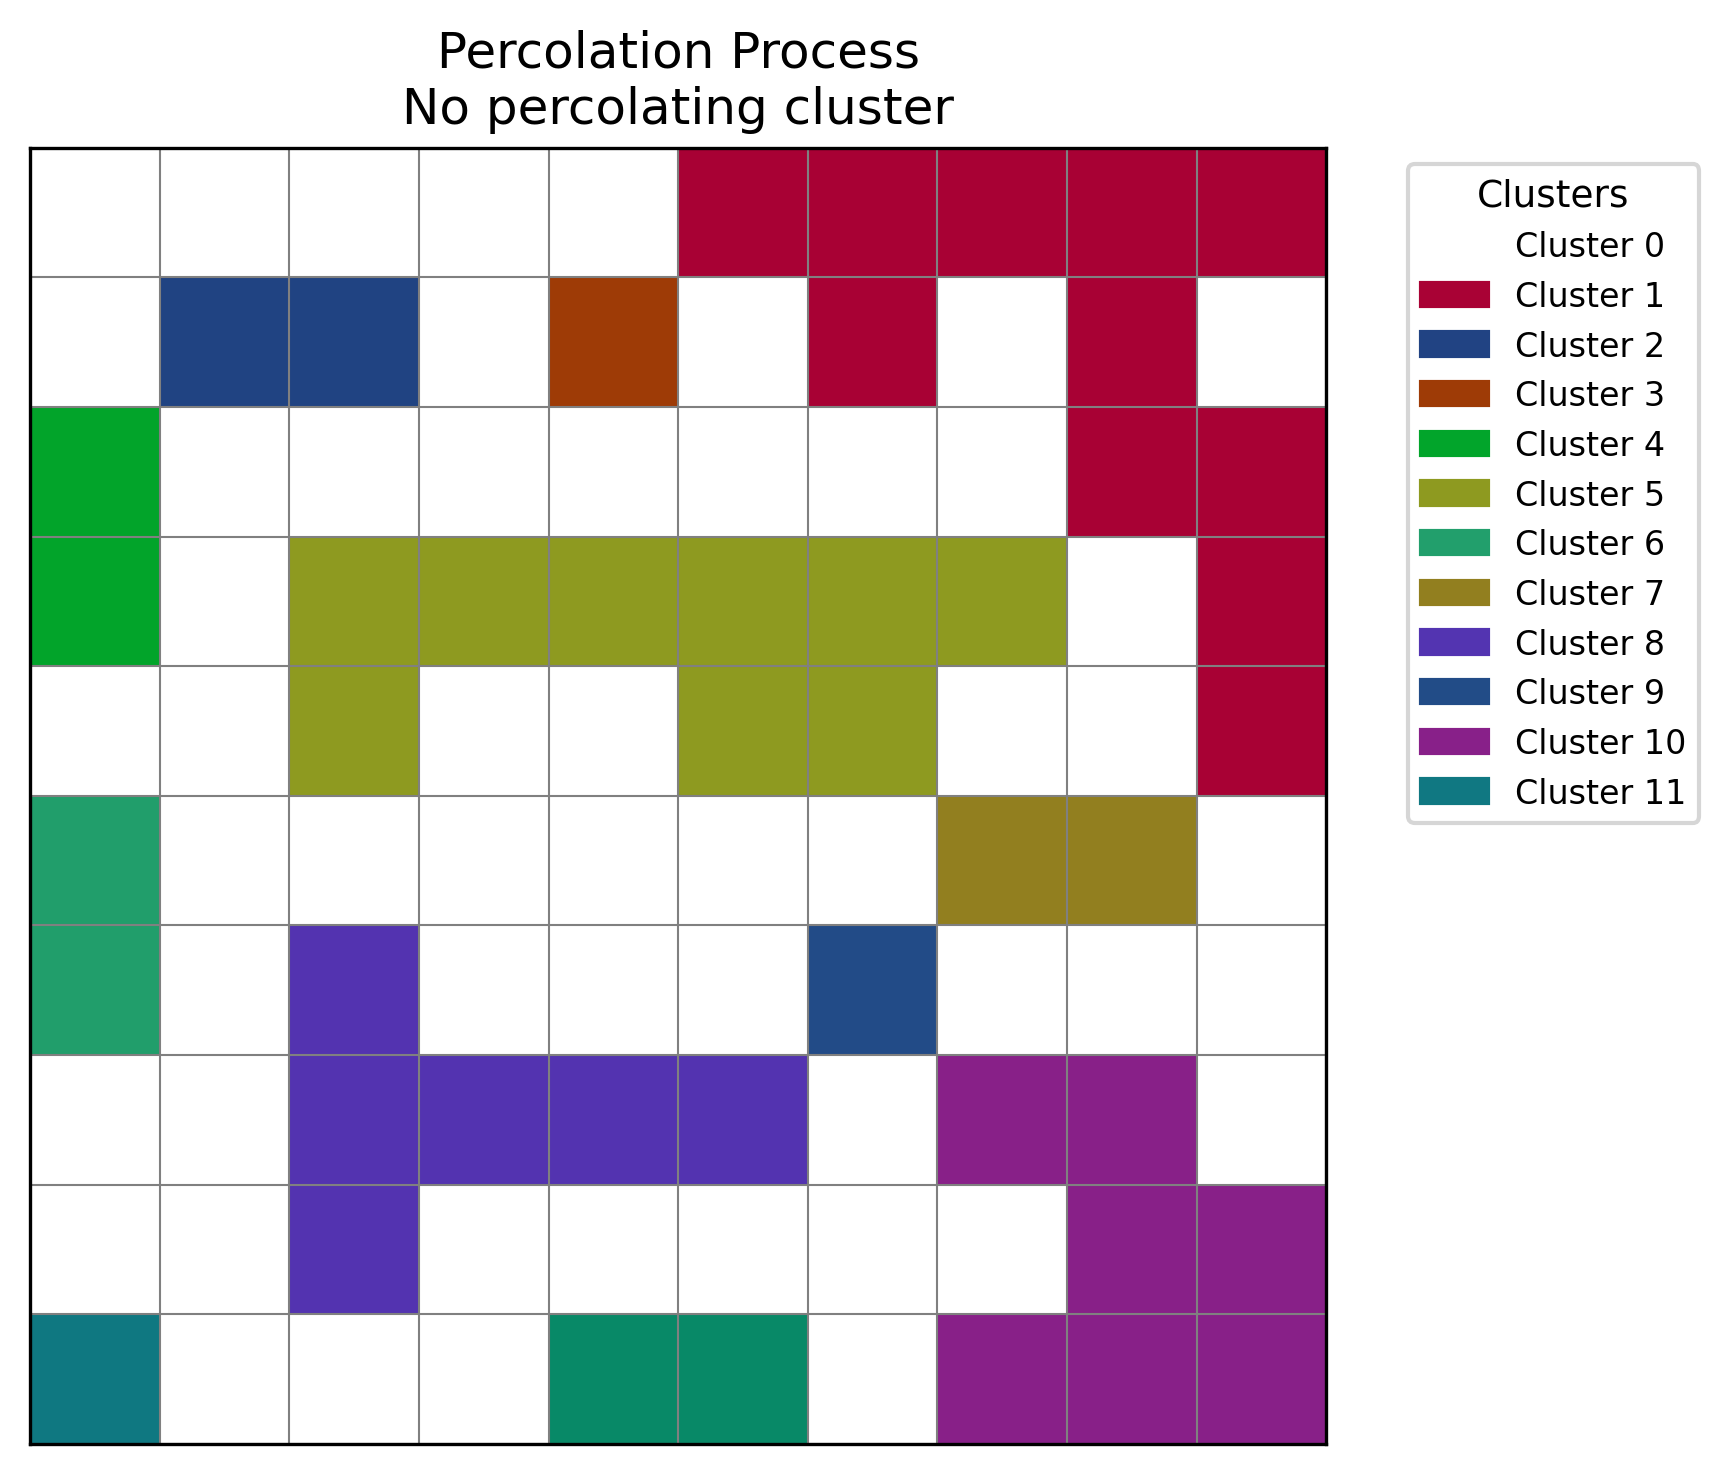
\includegraphics[width=0.7\textwidth]{../figures/clusterpercolation.png}
    \caption{Identificación de clusters individuales con diferentes colores. El cluster percolante se muestra en rojo.}
    \label{fig:cluster_vis}
\end{figure}

\section{Análisis de Escalamiento}

El comportamiento crítico se caracteriza por leyes de escalamiento de la forma:
\begin{align}
P(p,L) &\sim L^{-\beta/\nu} f_P\left((p-p_c)L^{1/\nu}\right) \\
S(p,L) &\sim (p-p_c)^{\beta} g_S\left((p-p_c)L^{1/\nu}\right)
\end{align}

donde $\nu \approx 4/3$ es el exponente de longitud de correlación y $f_P$, $g_S$ son funciones de escalamiento universales \cite{cardy1992scaling}.

\section{Conclusiones}

La implementación del algoritmo de Hoshen-Kopelman permite estudiar eficientemente el fenómeno de percolación en sistemas bidimensionales. Los resultados confirman:

\begin{itemize}
    \item El valor crítico $p_c \approx 0.5927$ para percolación de sitios en red cuadrada
    \item Comportamiento de escalamiento finito consistente con la teoría
    \item Formación de un cluster percolante dominante para $p > p_c$
    \item Dependencia del tamaño del sistema en las propiedades críticas
\end{itemize}

Este estudio proporciona una base sólida para investigaciones más avanzadas en teoría de percolación y fenómenos críticos.

\section{Agradecimientos}

Agradecemos al profesor del curso de Introducción a la Computación Científica de Alto Rendimiento por su guía en este proyecto.

% Bibliografía - CORREGIDO: cambiado de 'references' a 'report'
\bibliographystyle{unsrt}
\bibliography{report}

\end{document}